\section{Casi d'uso}

\subsection{Introduzione}
in questa sezione vengono presentati i casi d'uso individuati durante l'attività di analisi, 
condotta a partire dal capitolato d'appalto e dagli incontri con il proponente. 
Gli attori vengono identificati in base alla gerarchia trovata e 
alle funzionalità potenziali rilevate.

\subsubsection{Codifica dei casi d'uso}
I casi d'uso sono codificati utilizzando la seguente notazione:

\begin{itemize}
    \item \textbf{UC[ID-Principale][ID-Sottocaso]}: Identificativo univoco del caso d'uso, composto da un ID principale che identifica il caso principale e, se necessario, da un ID del sottocaso.
    \item \textbf{Titolo}: Breve descrizione del caso d'uso.
    \item \textbf{Attori}: Elenco degli attori coinvolti nel caso d'uso.
    \item \textbf{Precondizioni}: Condizioni che devono essere vere prima che il caso d'uso possa iniziare.
    \item \textbf{Postcondizioni}: Condizioni che devono essere vere dopo che il caso d'uso è stato completato con successo.
    \item \textbf{Scenario principale}: Descrizione dettagliata del flusso di eventi principale del caso d'uso.
    \item \textbf{Generalizzaioni}: Eventuali casi d'uso generalizzati.
    \item \textbf{Estensioni}: Eventuali casi d'uso estesi.
    \item \textbf{Inclusione:} Eventuali inclusioni
\end{itemize}
\newpage
\subsection{Casi d'uso}

\subsubsection{U.C.1 Utilizza chat} %%Esempio
\begin{itemize}
    \item \textbf{Attori}: Utente
    \item \textbf{Precondizioni}: Utente che ha acceduto nel sistema
    \item \textbf{Postcondizioni}: Utente ha effettuato una conversazione
    \item \textbf{Scenario principale}: L'utente vuole ricevere informazioni riguardanti "\textit{food/bevarage}" da acquistare per fornire la sua attività per farlo avvia una conversazione con il bot
    \item \textbf{Generalizzaioni}: U.C.1.1, U.C.1.2, U.C.1.3
    \item \textbf{Estensioni}: -
    \item \textbf{Inclusione:} -
\end{itemize}
\begin{figure}[h!]
    \centering
    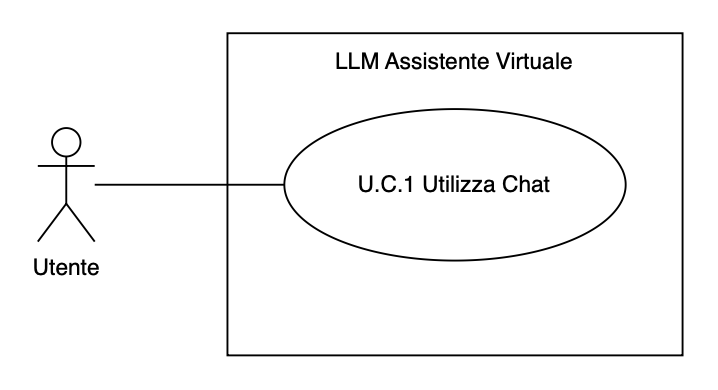
\includegraphics[width=0.5\textwidth]{img/UC1.png}
    \caption{U.C.1 Utilizza Chat}
\end{figure}
\begin{figure}[h!]
    \centering
    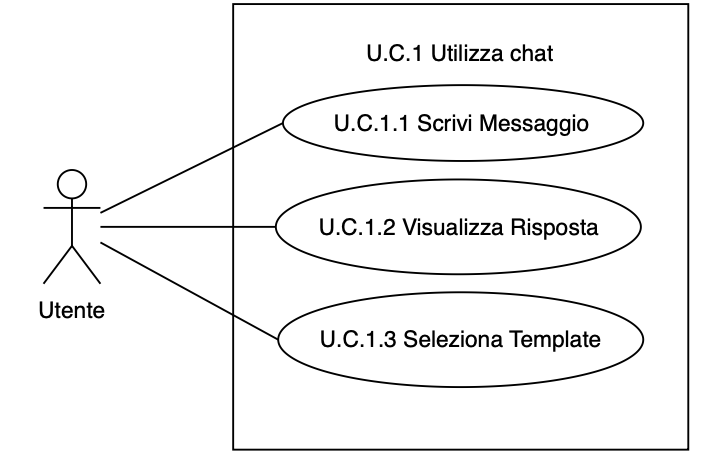
\includegraphics[width=0.5\textwidth]{img/SottocasiUC1.png}
    \caption{Sottocasi di U.C.1}
\end{figure}

\subsubsection{U.C.1.1 Scrivi Messaggio}
\begin{itemize}
    \item \textbf{Attori}: Utente
    \item \textbf{Precondizioni}: Utente che ha acceduto nel sistema ed è pronto per effetuare una domanda
    \item \textbf{Postcondizioni}: L'utente ha inviato un messaggio al bot
    \item \textbf{Scenario principale}: L’utente vuole domandare al bot delle informazioni riguardo un prodotto o una serie di prodotti
    \item \textbf{Generalizzaioni}: -
    \item \textbf{Estensioni}: -
    \item \textbf{Inclusione:} -
\end{itemize}
\subsubsection{U.C.1.2 Visualizza Risposta}
\begin{itemize}
    \item \textbf{Attori}: Utente
    \item \textbf{Precondizioni}: Utente che ha effettuato l'accesso ha inviato una domanda al bot
    \item \textbf{Postcondizioni}: Utente riceve una risposta dal bot coerente alla domanda che ha effettuato
    \item \textbf{Scenario principale}: L'utente che ha già effetuato la domanda per il bot riceve una risposta coerente sui prodotti
    \item \textbf{Generalizzaioni}: -
    \item \textbf{Estensioni}: -
    \item \textbf{Inclusione:} -
\end{itemize}
\subsubsection{U.C.1.4 Prodotto non trovato}
\begin{itemize}
    \item \textbf{Attori}: Utente
    \item \textbf{Precondizioni}: Utente che sta conversando con il bot
    \item \textbf{Postcondizioni}: L'assistente non ha trovato informazioni sul prodotto
    \item \textbf{Scenario principale}: L’utente richiede domande o informazioni su prodotti non gestiti da noi.
    \item \textbf{Generalizzaioni}: -
    \item \textbf{Estensioni}: -
    \item \textbf{Inclusione:} U.C.13
\end{itemize}
\begin{figure}[h!]
    \centering
    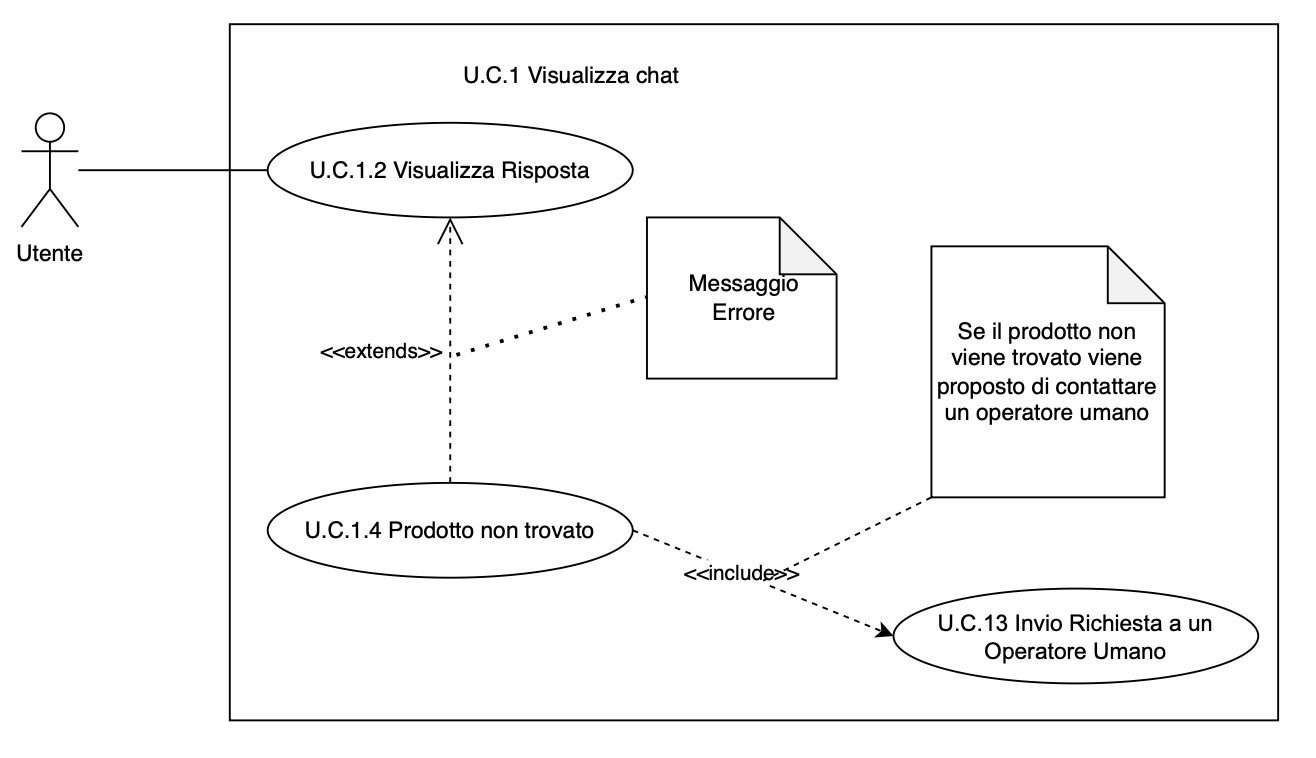
\includegraphics[width=0.8\textwidth]{img/UC1-4.png}
    \caption{U.C.1.4 Prodotto non trovato}
\end{figure}
\subsubsection{U.C.1.3 Seleziona Template}
\begin{itemize}
    \item \textbf{Attori}: Utente
    \item \textbf{Precondizioni}: Utente che ha effettuato l’accesso sta per selezionare un domanda templeatizzata 
    \item \textbf{Postcondizioni}: Utente ha ricevuto una risposta templeatizzata (\textit{senza dover chiamare l’LLM}).
    \item \textbf{Scenario principale}: L’utente dentro la chat vuole utilizzare una domanda templeatizzata tra le consigliate.
    \item \textbf{Generalizzaioni}: -
    \item \textbf{Estensioni}: -
    \item \textbf{Inclusione:} -
\end{itemize}
\subsubsection{U.C.2 Visualizza le conversazioni}
\begin{itemize}
    \item \textbf{Attori}: Utente
    \item \textbf{Precondizioni}: Utente che ha già effettuato l’accesso vuole visualizzare le conversazioni precedentemente salvate
    \item \textbf{Postcondizioni}: Utente vede una lista di conversazioni salvate
    \item \textbf{Scenario principale}: L’utente registrato che ha già effettuato una conversazione in passato salvandola vuole visualizzarla di nuovo in un secondo momento
    \item \textbf{Generalizzaioni}: -
    \item \textbf{Estensioni}: -
    \item \textbf{Inclusione:} U.C.2.1
\end{itemize}
\begin{figure}[h!]
    \centering
    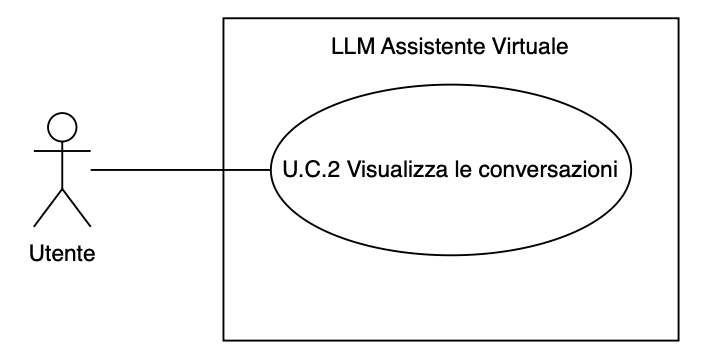
\includegraphics[width=0.5\textwidth]{img/UC2.png}
    \caption{U.C.2 Visualizza le conversazioni}
\end{figure}
\subsubsection{U.C.2.1 Visualizza conversazione singola}
\begin{itemize}
    \item \textbf{Attori}: Utente
    \item \textbf{Precondizioni}: Utente che ha già effettuato l’accesso seleziona una conversazione precedentemente salvata
    \item \textbf{Postcondizioni}: Utente vede la conversazione precedentemente effettuata
    \item \textbf{Scenario principale}: L’utente registrato che ha già effettuato una conversazione in passato salvandola vuole visualizzarla di nuovo in un secondo momento
    \item \textbf{Generalizzaioni}: U.C.2
    \item \textbf{Estensioni}: -
    \item \textbf{Inclusione:} -
\end{itemize}
\begin{figure}[h!]
    \centering
    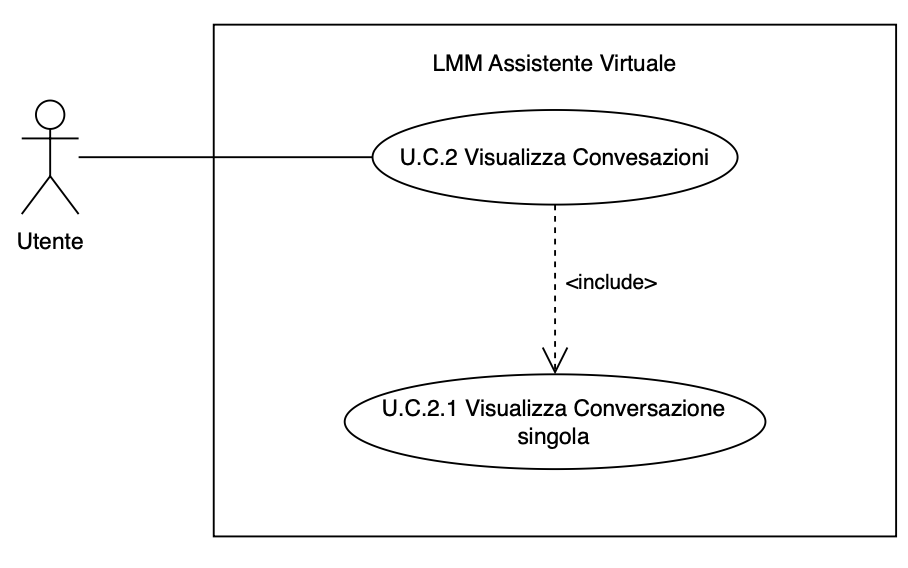
\includegraphics[width=0.6\textwidth]{img/UC2-1.png}
    \caption{U.C.2 Visualizza conversazione singola}
\end{figure}
\subsubsection{U.C.3 Login}
\begin{itemize}
    \item \textbf{Attori}: Utente
    \item \textbf{Precondizioni}: Utente già registrato
    \item \textbf{Postcondizioni}: Utente ha effettuato l'accesso
    \item \textbf{Scenario principale}: L'utente già registrato vuole accedere al sistema
    \item \textbf{Generalizzaioni}: -
    \item \textbf{Estensioni}: -
    \item \textbf{Inclusione:} -
\end{itemize}
\begin{figure}[h!]
    \centering
    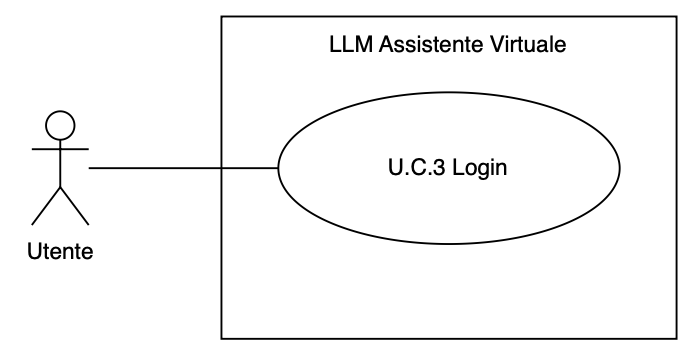
\includegraphics[width=0.5\textwidth]{img/UC3.png}
    \caption{U.C.3 Login}
\end{figure}
\begin{figure}[h!]
    \centering
    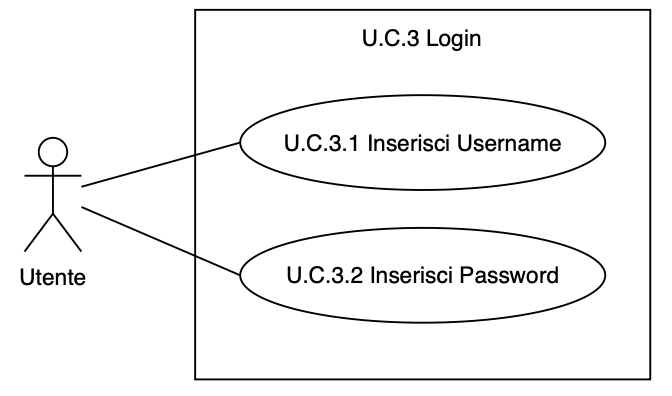
\includegraphics[width=0.5\textwidth]{img/UC3p1.png}
    \caption{Sottocasi di U.C.3}
\end{figure}
\subsubsection{U.C.3.1 Inserisci Username}
\begin{itemize}
    \item \textbf{Attori}: Utente
    \item \textbf{Precondizioni}: Utente già registrato
    \item \textbf{Postcondizioni}: Utente ha inserito un Username
    \item \textbf{Scenario principale}: L'utente già registrato vuole accedere al sistema
    \item \textbf{Generalizzaioni}: -
    \item \textbf{Estensioni}: U.C.3.4, U.C.3.5
    \item \textbf{Inclusione:} -
\end{itemize}
\subsubsection{U.C.3.4 Username errato}
\begin{itemize}
    \item \textbf{Attori}: Utente
    \item \textbf{Precondizioni}: Utente già registrato
    \item \textbf{Postcondizioni}: Utente ha inserito un username errato e gli viene impedito di accedere al sistema
    \item \textbf{Scenario principale}: L’utente ha provato ad accedere al sistema utilizzando un username errato e viene visualizzato un messaggio di errore generico
    \item \textbf{Generalizzaioni}: -
    \item \textbf{Estensioni}: -
    \item \textbf{Inclusione:} -
\end{itemize}
\begin{figure}[h!]
    \centering
    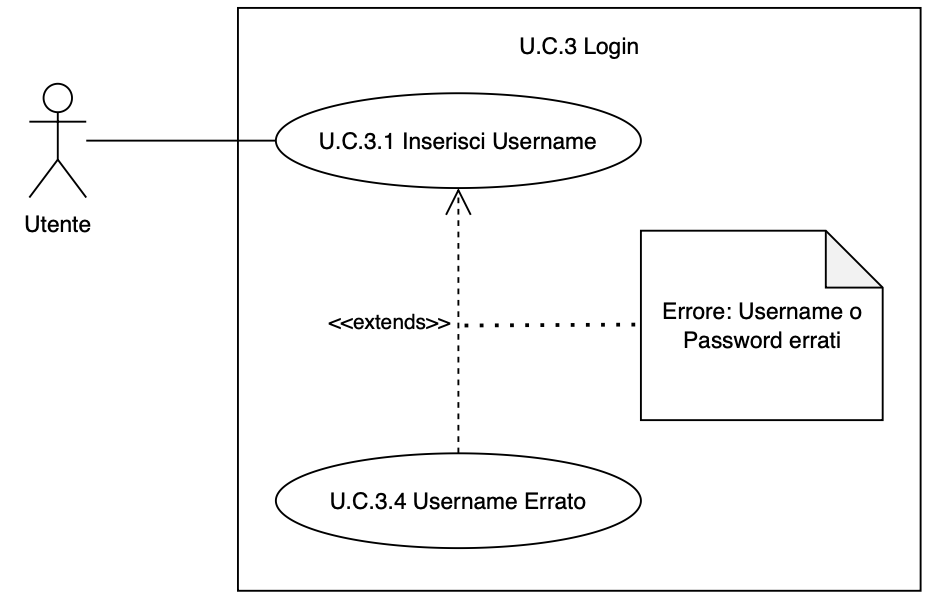
\includegraphics[width=0.6\textwidth]{img/UC3-4.png}
    \caption{U.C.3.4 Username errato}
\end{figure}
\subsubsection{U.C.3.2 Inserisci Password}
\begin{itemize}
    \item \textbf{Attori}: Utente
    \item \textbf{Precondizioni}: Utente già registrato
    \item \textbf{Postcondizioni}: Utente ha inserito una Password
    \item \textbf{Scenario principale}: L'utente già registrato vuole accedere al sistema
    \item \textbf{Generalizzaioni}: -
    \item \textbf{Estensioni}: U.C.3.3, U.C.3.5
    \item \textbf{Inclusione:} -
\end{itemize}
\subsubsection{U.C.3.3 Password Errata}
\begin{itemize}
    \item \textbf{Attori}: Utente
    \item \textbf{Precondizioni}: Utente già registrato
    \item \textbf{Postcondizioni}: Utente ha inserito una Password errata e gli viene impedito di accedere al sistema
    \item \textbf{Scenario principale}: L'utente ha provato ad accedere al sistema utilizzando una Password errata e viene visualizzato un messaggio di errore generico
    \item \textbf{Generalizzaioni}: -
    \item \textbf{Estensioni}: -
    \item \textbf{Inclusione:} -
\end{itemize}
\begin{figure}[h!]
    \centering
    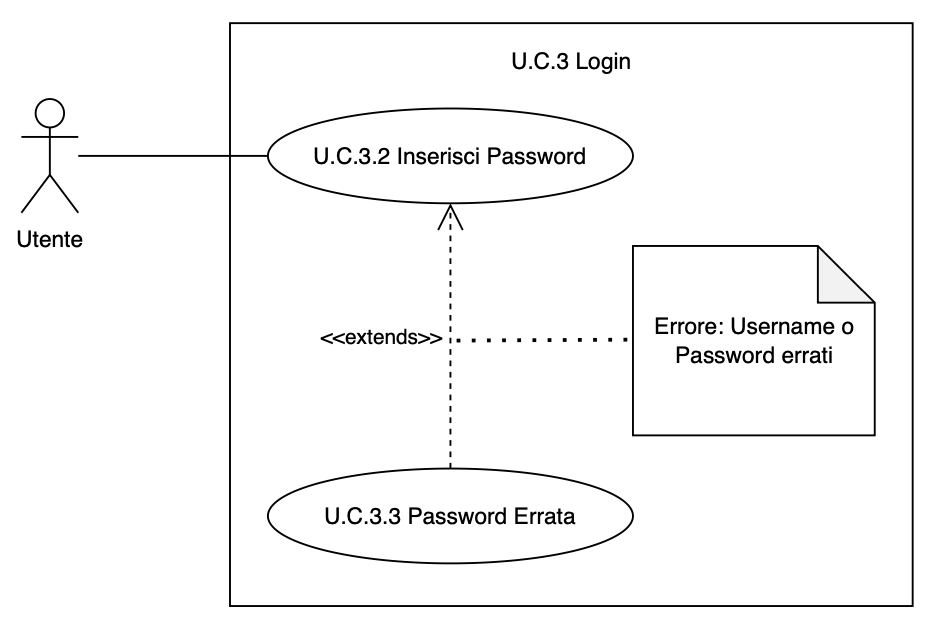
\includegraphics[width=0.7\textwidth]{img/UC3-3.png}
    \caption{U.C.3.3 Password errato}
\end{figure}
\subsubsection{U.C.3.5 Caratteri non validi}
\begin{itemize}
    \item \textbf{Attori}: Utente
    \item \textbf{Precondizioni}: Utente già registrato
    \item \textbf{Postcondizioni}: Utente ha inserito caratteri particolari e gli viene impedito di accedere al sistema
    \item \textbf{Scenario principale}: L’utente ha provato ad entrare nel sistema cercando di rompere o rubare informazioni e gli viene impedito di entrare nel sistema
    \item \textbf{Generalizzaioni}: -
    \item \textbf{Estensioni}: -
    \item \textbf{Inclusione:} -
\end{itemize}
\begin{figure}[h!]
    \centering
    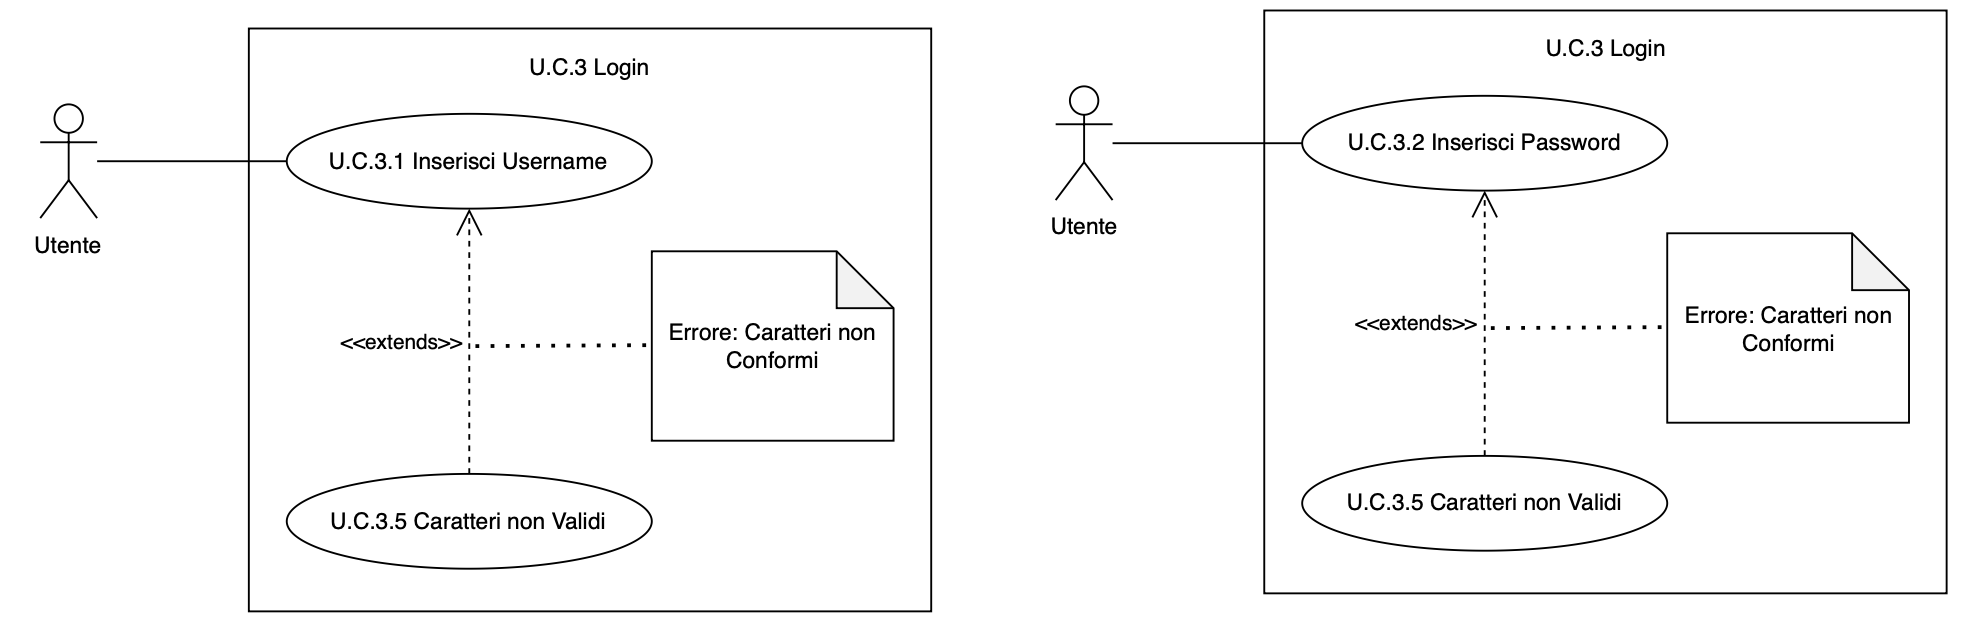
\includegraphics[width=\textwidth]{img/UC3-5.png}
    \caption{U.C.3.5 Caratteri non validi}
\end{figure}